\documentclass[11pt]{ujarticle}
%\documentclass{jlreq,11pt}
%%%%%%% スタイルファイル %%%%%%%%%%%%%%%%%%%%%%
\usepackage{amsmath,amssymb}

\usepackage{thesis}

\usepackage[dvipdfmx]{graphicx}   % pdf 形式の図版取り込みのため
\usepackage[dvipdfmx]{color}
\usepackage{ascmac}
\usepackage{multicol}

\usepackage{float}
\usepackage{indent}
\usepackage{url}

\usepackage{color}
\definecolor{lightgray}{gray}{0.9}
\definecolor{darkgray}{gray}{0.25}

\usepackage{framed}
\makeatletter
\renewenvironment{leftbar}{%
  \def\FrameCommand{\hspace{1.5zw}\textcolor{darkgray}{\vrule width 2pt}\hspace{0.5zw}}% 
  \MakeFramed {\advance\hsize-\width \FrameRestore}}%
 {\endMakeFramed}
\makeatother

\usepackage[dvipdfmx]{graphicx}
\usepackage{listings,jlisting}
\usepackage{mylistings}

\lstset{
  basicstyle={\ttfamily},
  identifierstyle={\small},
  commentstyle={\smallitshape},
  keywordstyle={\small\bfseries},
  ndkeywordstyle={\small},
  stringstyle={\small\ttfamily},
  frame={tb},
  breaklines=true,
  columns=[l]{fullflexible},
  numbers=left,
  xrightmargin=0zw,
  xleftmargin=3zw,
  numberstyle={\scriptsize},
  stepnumber=1,
  numbersep=1zw,
  lineskip=-0.5ex
}

\begin{document}

%%%%%%%%%%%%%%%%%%%%%%%%%%%%%%%%%%%%%%%%%%%%%%%%%%%%%%%%%%%%%%%%%%%%%%%%%%%%%
%%%%%% 表紙 %%%%%%%%%%%%%%%%%%%%%%%%%%%%%%%%%%%%%%%%%%%%%%%%%%%%%%%%%%%%%%%
%%%%%%%%%%%%%%%%%%%%%%%%%%%%%%%%%%%%%%%%%%%%%%%%%%%%%%%%%%%%%%%%%%%%%%%%%%%%%

% === 年度を記入 ============================================================
\def\year{1}	% 令和 1 年度の場合

% === 提出年月日を記入 ============================================================
\def\submityear{2}	% 令和 2 年
\def\submitmonth{2}	% 2 月
\def\submitdate{4}	% 4 日

% === 題目を記入 ============================================================
\def\title{%
小型衛星模型を用いた磁気トルカによる姿勢制御の検証
}%

% === 題目を記入(背表紙用) ============================================================
\def\spine{%
小型衛星模型を用いた磁気トルカによる姿勢制御の検証
}%

% === 学科を記入 ==========================================================
\def\course{電子制御工学科}

% === 学籍番号を記入 ========================================================
\def\student_number{s9122}

% === 氏名を記入 ============================================================
\def\name{西保 洸太}

% === 指導教員を記入 ========================================================
\def\supervisor{{西 佑介 准教授}}

% === 表紙 ========================================================
\thispagestyle{empty}
% % !TEX root = main.tex


{\renewcommand{\arraystretch}{0.5}
\begin{tabular}{|p{16.5cm}|}
\hline
{\scriptsize{舞鶴工業高等専門学校 電子制御工学科 卒業論文 (令和\ \submityear\ 年\ \submitmonth\ 月\ \submitdate\ 日提出)}}\\
{\small\bf{\spine}}\\
\hfill\scriptsize\bf{\name (\student_number)}
\\
\hline
\end{tabular}}

\newpage
% ======================================================================
\begin{center}
{\fontsize{20pt}{0pt}\selectfont\bf{令和\ 6\ 年度}}\\[1zh]
{\fontsize{28pt}{0pt}\selectfont\bf{\kintou{8zw}{卒業研究論文}}}
\end{center}
% ======================================================================
\vspace{2zh}


% ======================================================================
\begin{center}
\fontsize{20pt}{26pt}\selectfont
\renewcommand{\arraystretch}{1.4}
\begin{tabular}{|p{2zw}|p{20zw}|}
\hline
{\bf{題目}} &
{\bf{\title}}\\\hline
\end{tabular}
\end{center}
% ======================================================================
\vspace{2zh}

% ======================================================================
\begin{center}
\fontsize{16pt}{18pt}\selectfont
\renewcommand{\arraystretch}{1.4}
\tabcolsep 4pt
\begin{tabular}{|p{4zw}|p{14zw}|}
\hline
{\bf{\kintou{4zw}{学科}}} &
{\bf{\course}}\\\hline
{\bf{\kintou{4zw}{学籍番号}}} &
{\bf{\student_number}}\\\hline
{\bf{\kintou{4zw}{氏名}}} &
{\bf{\name}}\\\hline
{\bf{\kintou{4zw}{提出日}}} &
{\bf{令和\ \submityear\ 年\ \submitmonth\ 月\ \submitdate\ 日}}\\\hline
\end{tabular}
\end{center}
% ======================================================================
\vspace{0zh}

% ======================================================================
\begin{center}
\fontsize{16pt}{18pt}\selectfont
\renewcommand{\arraystretch}{1.4}
\tabcolsep 4pt
\begin{tabular}{|p{4zw}|p{14zw}|}
\hline
{\bf{\kintou{4zw}{指導教員}}} &
{\bf{\supervisor}}\\\hline
\end{tabular}
\end{center}
% ======================================================================

\vfill
% ======================================================================
\begin{center}

\includegraphics[width=45mm]{figure/logo_maizuru_gray.pdf}
\end{center}
% ======================================================================
\vspace{0.25zh}
% ======================================================================
\begin{center}
{\fontsize{22pt}{0pt}\selectfont\bf{舞鶴工業高等専門学校}}\\[1zh]
{\fontsize{22pt}{0pt}\selectfont\bf{電子制御工学科}}
\end{center}
% ======================================================================


 \newpage

% === 論文要旨 ========================================================
\thispagestyle{empty}
% % !TEX root = main.tex
\begin{center}
\section*{論\,文\,要\,旨}                      %% ここに番号をつけない
\end{center}

 ここには論文要旨を書きます.
ここには論文要旨を書きます.
ここには論文要旨を書きます.
ここには論文要旨を書きます.
ここには論文要旨を書きます.
ここには論文要旨を書きます.
ここには論文要旨を書きます.
ここには論文要旨を書きます.
ここには論文要旨を書きます.
ここには論文要旨を書きます.
ここには論文要旨を書きます.
ここには論文要旨を書きます.
ここには論文要旨を書きます.
ここには論文要旨を書きます.
ここには論文要旨を書きます.
ここには論文要旨を書きます.
ここには論文要旨を書きます.
ここには論文要旨を書きます.
ここには論文要旨を書きます.
ここには論文要旨を書きます.
ここには論文要旨を書きます.
 \newpage

%%%%%%%%%%%%%%%%%%%%%%%%%%%%%%%%%%%%%%%%%%%%%%%%%%%%%%%%%%%%%%%%%%%%%%%%%%%%%
%%%%%% 目次 %%%%%%%%%%%%%%%%%%%%%%%%%%%%%%%%%%%%%%%%%%%%%%%%%%%%%%%%%%%%%%%
%%%%%%%%%%%%%%%%%%%%%%%%%%%%%%%%%%%%%%%%%%%%%%%%%%%%%%%%%%%%%%%%%%%%%%%%%%%%%
\pagenumbering{roman}
% \tableofcontents         %% 目次 
\newpage

\pagenumbering{arabic}
\setcounter{page}{1}
%%%%%%%%%%%%%%%%%%%%%%%%%%%%%%%%%%%%%%%%%%%%%%%%%%%%%%%%%%%%%%%%%%%%%%%%%%%%%
%%%%%% 本文 %%%%%%%%%%%%%%%%%%%%%%%%%%%%%%%%%%%%%%%%%%%%%%%%%%%%%%%%%%%%%%%
%%%%%%%%%%%%%%%%%%%%%%%%%%%%%%%%%%%%%%%%%%%%%%%%%%%%%%%%%%%%%%%%%%%%%%%%%%%%%
% !TEX root = main.tex
%%%%%%%%%%%%%%%%%%%%%%%%%%%%%%%%%%%%%%%%%%%%%%%%%%%%%%
\section{序論}
%%%%%%%%%%%%%%%%%%%%%%%%%%%%%%%%%%%%%%%%%%%%%%%%%%%%%%
\subsection{始めに}
人工衛星とは,地球の周りをまわっている人工物体のことをいい,搭載しているセンサなどで地球の気象や地上の状況を調べる地球観測衛星,
位置情報を正確に測る測位衛星,インターネットなどを構成する通信衛星などがある.
2023年に打ち上げられた人工衛星等の機数は,過去最大の2,901機であり,10年前と比べて約14倍に増加した.
数十~数千の人工衛星を一体的に運用しネットワークを構築する,メガコンステレーションの構築への取り組みや,
先進国による宇宙利用への期待の高まりから,宇宙輸送のニーズは一層拡大することが見込まれている.

 人工衛星は,大きいものでは例えばISS(国際宇宙ステーション)がある.
それに対し小さいものでは,一辺10cmの立方体サイズの超小型人工衛星が存在している.

 大型人工衛星,中型人工衛星と呼ばれる人工衛星は,多くが国家プロジェクトとして開発され,打ち上げられている.
その特徴として,高機能で信頼性が高く,複雑な用途,複数のミッションに活用できるという利点がある.
しかし,設計・製造に莫大な費用と時間が必要となる.

 それに対し,超小型人工衛星は,機能が制限され,単一のミッションしか実行できないという欠点がある.
その代わり,短期間での開発・低コストでの打ち上げが可能であるため,
学生,大学院生が在学中に開発・打ち上げをすることが可能となっている.
また,世界各国が宇宙開発研究でしのぎを削るなか,新しい技術を素早く試せることも,
注目されている一つの理由である.

超小型人工衛星での姿勢制御は,地球観測や高速通信といったミッションで応用される.

 超小型人工衛星は,その小ささから,搭載可能な機器のサイズや重量に制限がある.
そのため,リアクションホイールやスラスタといった,性能の代わりに大型な機器は搭載が難しい.
そこで,姿勢制御に磁気トルカと呼ばれる電磁石が用いられることが多い.



\subsection{本研究の目的}
 人工衛星の姿勢制御を地上で実験し,研究・検討するには,通常球面の空気軸受けを使った3軸テーブルが用いられる.
しかし,3軸で制御する衛星でも,3軸を同時に制御する状態は必要とせず,1軸のみでの制御実験を先に検証する場合が多い.
また,3軸テーブルでの実験の設計の難しさから,1軸テーブルは有効な実験道具となる.

本研究では,小型衛星の模型を用いて,磁気トルカで衛星の姿勢制御を行う様子を再現し, \newpage
% % !TEX root = main.tex
%%%%%%%%%%%%%%%%%%%%%%%%%%%%%%%%%%%%%%%%%%%%%%%%%%%%%%
\section{制御理論}

\subsection{本研究で用いる理論}
本研究では,P制御,P-D制御,B-dot制御則,クロスプロダクト則を検証する.

本研究で用いる制御モデルは,電流Iを入力とし,出力は角度$\theta$である.
この二つの関係を運動方程式で表すと,

\begin{equation}
    \begin{aligned}
        J\ddot{\theta} &= \boldsymbol{M \times B}\\
                       &= MB\sin\theta\\
                       &= \mu nISB\sin\theta
    \end{aligned}
\end{equation}

となり,線形事変システムであるため,モデル化が難しい.
そのためP制御,PD制御では,
制御対象のモデリングを必要としない,
限界感度法を用いてゲインの調整を行った.



%%%%%%%%%%%%%%%%%%%%%%%%%%%%%%%%%%%%%%%%%%%%%%%%%%%%%%
\subsection{P制御}
%%%%%%%%%%%%%%%%%%%%%%%%%%%%%%%%%%%%%%%%%%%%%%%%%%%%%%




%%%%%%%%%%%%%%%%%%%%%%%%%%%%%%%%%%%%%%%%%%%%%%%%%%%%%%
\subsection{P-D制御}
%%%%%%%%%%%%%%%%%%%%%%%%%%%%%%%%%%%%%%%%%%%%%%%%%%%%%%
\newpage
%%%%%%%%%%%%%%%%%%%%%%%%%%%%%%%%%%%%%%%%%%%%%%%%%%%%%%
\subsection{B-dot制御則}
%%%%%%%%%%%%%%%%%%%%%%%%%%%%%%%%%%%%%%%%%%%%%%%%%%%%%%
 B-dot制御則とは,人工衛星のある1軸を規定し,その軸に沿った磁場の変化率の符号と反対の磁気モーメントを発生させる制御である.

 静止状態において,地磁気ベクトル$\boldsymbol{B}_\mathrm{geo}$が,衛星を基準とするx-y平面上のx軸に沿っていると考えると,
t秒後の地磁気のx成分$B_x$,y成分$B_y$は,地磁気ベクトルの大きさ$B_o=|\boldsymbol{B}_\mathrm{geo}|$,角速度$\omega_z$を用いて,
\begin{align}
    \left\{
        \begin{aligned}
            B_x &= B_o\cos\omega_zt\\
            B_y &= -B_o\sin\omega_zt\\
        \end{aligned}                    
    \right.
\end{align}

で表される.
そして,それぞれの時間変化は,

\begin{align}
    \left\{
        \begin{aligned}
            \dot{B_x} &= -B_o\omega_z\sin\omega_zt = B_y\omega_z\\
            \dot{B_y} &= -B_o\omega_z\cos\omega_zt = -B_x\omega_z
        \end{aligned}                    
    \right.
\end{align}

である.
初期位相および目標角を0 [deg] とすると,目標磁気モーメントは

\begin{equation}
    M_x = -k\dot{B_x} = -B_o\omega_z\sin\omega_zt
\end{equation}

で決定される.
このとき,生じるトルクは,
\begin{equation}
    \begin{aligned}
        \mathrm{T_z} &= M_x \times B_y\\
                     &= (kB_o\omega_z\sin\omega_zt)(-B_o\sin\omega_zt)\\
                     &= -kB_o^2\omega_z\sin^2\omega_zt
    \end{aligned}
\end{equation}

である.
衛星の1回転にわたり,$\sin\omega_zt$の平均値は0.5となるため,その平均値は

\begin{equation}
    \mathrm{T_\mathrm{z,ave}} = \frac{-kB_o^2\omega_z}{2}
\end{equation}

で表される.このトルクから,衛星の回転運動についての運動方程式は,

\begin{equation}
    I_z\dot{\omega_z} = \dot{L} = \mathrm{T_\mathrm{z,ave}} = \frac{-kB_o^2\omega_z}{2}
\end{equation}

となる.これを変形して,

\begin{equation}
    \dot{\omega_z}+\frac{kB_o^2}{2I_z}\omega_z = 0
\end{equation}

が得られる.この微分方程式は,$\tau=\frac{I_z}{kB_o^2}$とすると,

\begin{equation}
    \omega_z = \omega_{z_o}e^{-\frac{t}{2\tau}} 
\end{equation}

となり,指数関数的に角速度が減少することがわかる.\\
 次に,磁気トルカを1つ増やし,それをy軸に添わせることを考える.
目標磁気モーメントは

\begin{equation}
    M_x = -k\dot{B_y} = kB_o\omega_z\cos\omega_zt
\end{equation}

となる.
二つの磁気トルカにより生じるトルクを合成すると,

\begin{equation}
    \begin{aligned}
        T_z &= M_xB_y - M_yB_x\\
            &= (kB_o\omega_z\sin\omega_zt)(-B_o\sin\omega_zt)-(kB_o\omega_z\cos\omega_zt)(B_o\cos\omega_zt)\\
            &= -kB_o^2\omega_z\sin^2\omega_zt - kB_o^2\omega_z\cos^2\omega_zt\\
            &= -kB_o^2\omega_zt\\
            &= \dot{L} = I_Z\dot{\omega_z}
    \end{aligned}
\end{equation}

この微分方程式の$\omega_z$の解は,

\begin{equation}
    \omega_z = \omega_{z_o}e^{-\frac{t}{\tau}} 
\end{equation}

となるので,減衰の時定数が半分となることがわかる.
 次に,磁気トルカをもう1つ追加したときを考える.3つの磁気トルカがそれぞれ直交するように衛星に配置されているとき,
x-y平面,z-x平面,y-z平面について,B-dot制御を考える.
x軸回り,y軸回りの角速度を$\omega_x$,$\omega_y$とすると,

\begin{align}
    \left\{
        \begin{aligned}
            B_z &= B_o\cos\omega_yt\\
            B_x &= -B_o\sin\omega_yt\\
        \end{aligned}                    
    \right.
    ,
    \left\{
        \begin{aligned}
            B_y &= B_o\cos\omega_xt\\
            B_z &= -B_o\sin\omega_xt\\
        \end{aligned}                    
    \right.
\end{align}

で表される.
そして,それぞれの時間変化は,

\begin{align}
    \left\{
        \begin{aligned}
            \dot{B_z} &= -B_o\omega_y\sin\omega_yt = B_x\omega_y\\
            \dot{B_x} &= -B_o\omega_y\cos\omega_yt = -B_z\omega_y
        \end{aligned}                    
    \right.
    ,
    \left\{
        \begin{aligned}
            \dot{B_y} &= -B_o\omega_x\sin\omega_xt = B_z\omega_x\\
            \dot{B_z} &= -B_o\omega_x\cos\omega_xt = -B_y\omega_x
        \end{aligned}                    
    \right.
\end{align}

となる.(1.2)式と(1.13)式を重ね合わせると,

\begin{equation}
    \left\{
        \begin{aligned}
            \dot{B_x} = B_y\omega_z - B_z\omega_y\\
            \dot{B_y} = B_z\omega_x - B_x\omega_z\\
            \dot{B_z} = B_x\omega_y - B_y\omega_x
        \end{aligned}
    \right.
\end{equation}

となることから,xyz空間において,地磁気の時間変化は

\begin{equation}
    \boldsymbol{\dot{B} = B \times \omega}
\end{equation}

で表され,
目標磁気モーメントは,

\begin{equation}
    \begin{aligned}
        \boldsymbol{M} &= -k \boldsymbol{\dot{B}}\\
                       &= -k(\boldsymbol{B \times \omega})
    \end{aligned}
\end{equation}

で求められる.

\subsection{クロスプロダクト則}
 衛星座標系で測定された地磁気ベクトル$\boldsymbol{b_m}$,その衛星の位置が目標姿勢を保っていた場合の地磁気ベクトル$\boldsymbol{b_r}$を用いて,
外積ベクトル$\boldsymbol{c}$を

\begin{equation}
    \boldsymbol{c} = \boldsymbol{\frac{b_m}{|b_m|}\times\frac{b_r}{|b_r|}}
\end{equation}

で定める.
これと,角速度の誤差$\Delta\omega = [\omega_x\space\omega_y\space\omega_z]$を用いて,
目標トルクが

\begin{equation}
    \boldsymbol{T}_R = K\boldsymbol{c}+k\Delta\boldsymbol{\omega}\\
\end{equation}

で定められる.なお,$K,k$は,

\begin{equation}
    K = 
    \begin{bmatrix}
        K_x & 0 & 0 \\
        0 & K_y & 0 \\
        0 & 0 & K_z \\
    \end{bmatrix}
    ,k =
    \begin{bmatrix}
        k_x & 0 & 0 \\
        0 & k_y & 0 \\
        0 & 0 & k_z \\
    \end{bmatrix}
\end{equation}

で定められる係数行列である.
本研究はz軸方向の一軸のみ制御するため,$c_z = b_{m_x}b_{r_y} - b_{m_y}b_{r_x}$なので,

\begin{equation}
    T_{R_z} = K_x c_z + k_x \omega_z 
\end{equation}

で,
磁気トルカにより発生するトルクの式より,磁気トルカの目標磁気モーメントは,

\begin{equation}
    \begin{aligned}
        T_z = M_x B_y - M_y B_x &= M_x B_y (なお,M_y = 0)\\
         K_x c_z + k_x \omega_z &= M_x B_y\\
                            M_x &= \frac{K_x c_z + k_x \omega_z}{B_y}
    \end{aligned}
\end{equation}

で求められる. \newpage
% !TEX root = main.tex
%%%%%%%%%%%%%%%%%%%%%%%%%%%%%%%%%%%%%%%%%%%%%%%%%%%%%%
\section{実験システムの構築}
%%%%%%%%%%%%%%%%%%%%%%%%%%%%%%%%%%%%%%%%%%%%%%%%%%%%%%
\subsection{構造}
 本研究では,図\ref{fig:system}に示すような超小型人工衛星の模型を用いて実験を行う.
模型は,転がり軸受を利用してできるだけ滑らかに回転し,各制御理論の特性が摩擦の影響を受けることなくなるべく反映されるようになっている.
人工衛星に搭載している物は,Arduino Uno,SD Cardシールド,磁気・角度・角速度センサ,磁気トルカ駆動用の回路,磁気トルカ,9 V 角型乾電池である.
Arduinoへの電力供給は角型乾電池を用い,磁気トルカへの電力供給は菊水電子工業株式会社製のPMC18-5Aを用いる.

\begin{figure}[H]
	\centering
		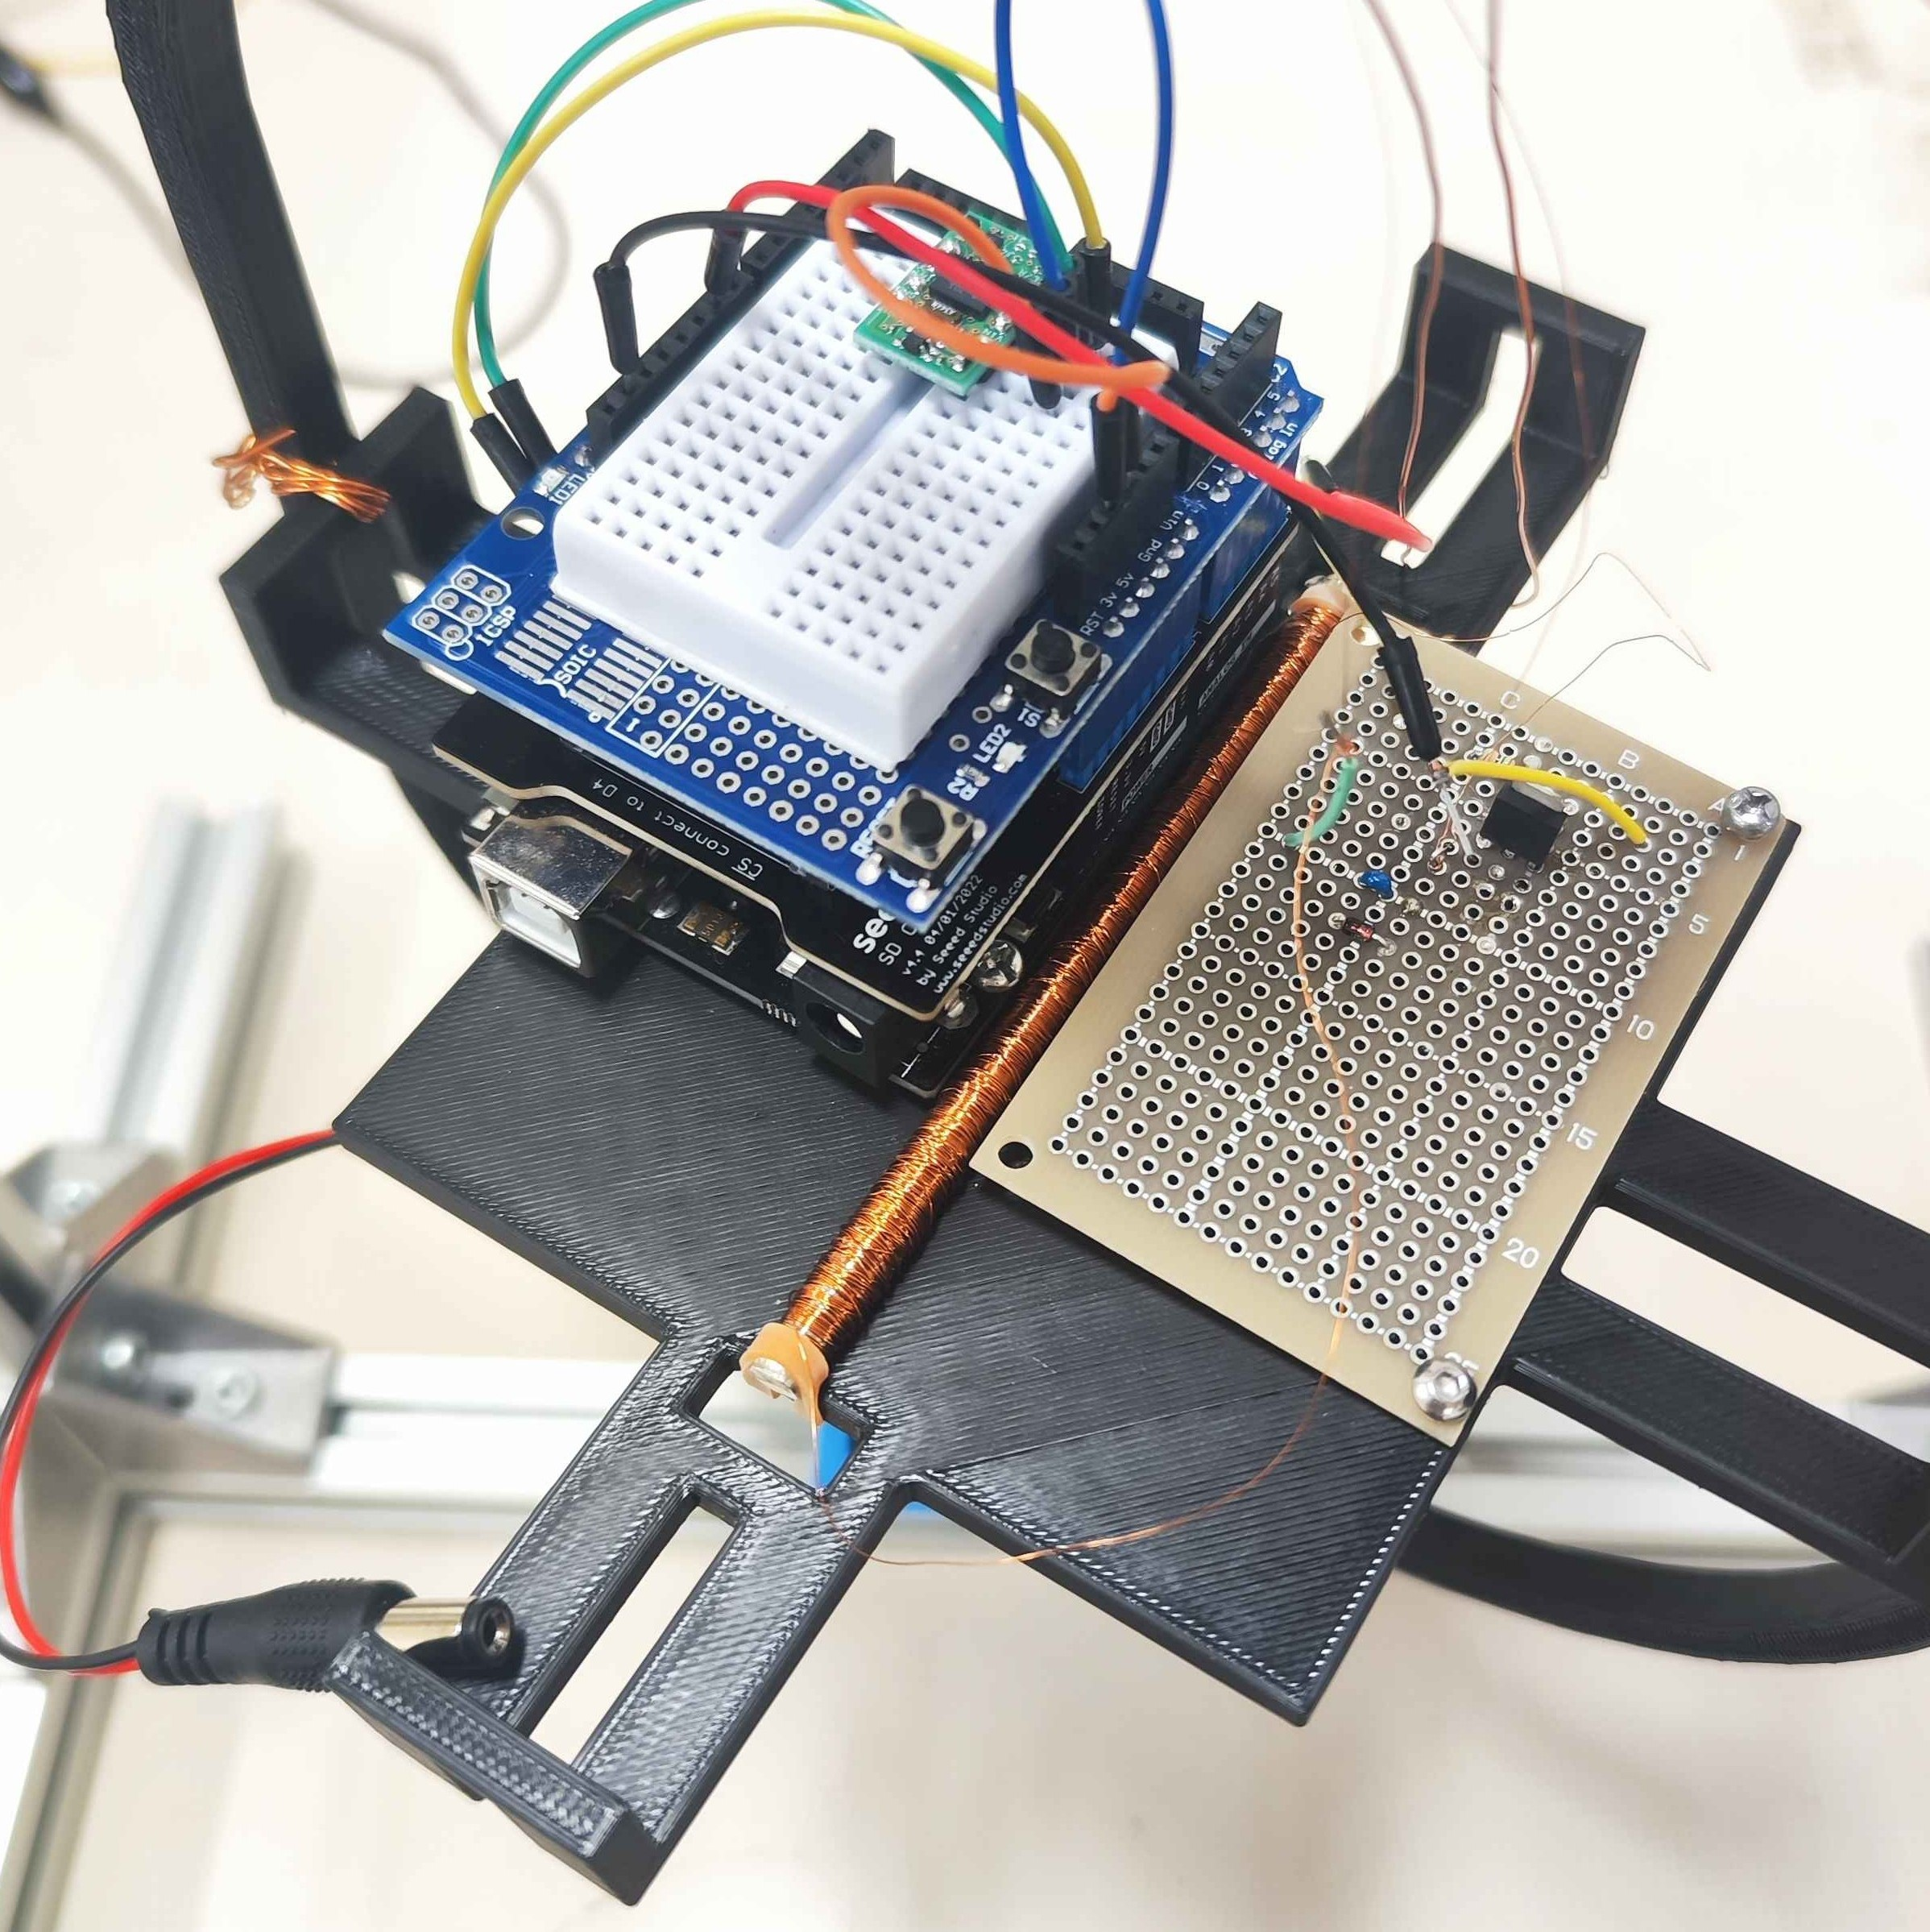
\includegraphics[scale=0.1]{./figure/実験システム.jpg}
		\caption{実験システムの外観}
		\label{fig:system}
\end{figure}

\subsection{制御システムの設計}

 搭載するArduinoは,ELEGOO社製のArduino Uno R3を,開発環境にはArduino IDEを用いる.
姿勢角度,角速度および磁力の検出には,Bosch Sensortec社のBNO055と,
Arduino IDEのライブラリ$"\mathrm{Adafruit\_Sensor.h}"$,$"\mathrm{Adafruit\_BNO055.h}"$
を用いる.また,姿勢角度,角速度および磁力の記録にはSDカードを用いており,
seeed studio社製のSD Card shield V4.0をArduinoに装着している.
センサから取得した角度,角速度および磁気のデータを用いて,フィードバック制御を行う.
記録した角度・角速度のデータをCSVファイルに保存,それをPythonでグラフに描画し,姿勢角度の遷移を確認する.

\begin{figure}[H]
	\centering
		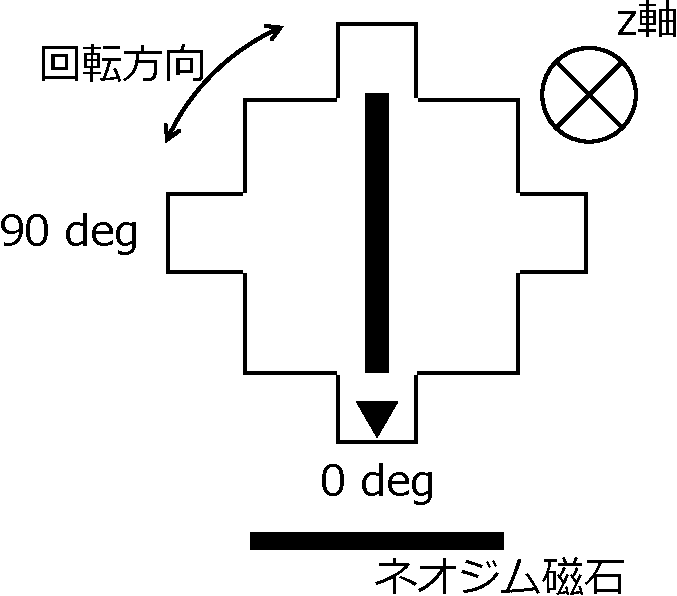
\includegraphics[scale=0.5]{./figure/system-crop.pdf}
		\caption{実験システム概略図}
		\label{fig:systemfig}
\end{figure}

\subsubsection{磁気トルカの制作}

 搭載した磁気トルカのパラメータを表\ref{table:torquer}に示す.
$\boldsymbol{E-B}$対応において,磁気トルカが発生させる磁気モーメントは,電流$I$,磁心の断面積$S$,法線ベクトル$\boldsymbol{n}$を用いて,
\begin{equation}
	\boldsymbol{m}=IS\boldsymbol{n}
\end{equation}
と表される.また,地磁気を$\boldsymbol{B}_\mathrm{geo}$ [T] とすると,磁気トルカがとらえる磁束密度は,
\begin{equation}
	\boldsymbol{B} = \mu_r\boldsymbol{B}_\mathrm{geo}
\end{equation}
となる.
そして,磁気トルカが発生させられるトルクは,磁気トルカの磁気モーメントと,磁気トルカがとらえる磁束密度を用いて,
\begin{equation}
	\boldsymbol{T = m \times B}
\end{equation}
と表される.

 まず,芯材にステンレス鋼を用いて磁気トルカを作り,磁石を用いて反応性を確かめた.
しかし,ステンレス鋼の保磁力の高さのため,磁気トルカに電流を流していないときも磁力を持っており,
また比透磁率も低く,電流を流しているとき,いないときの差がなく磁力も低かったため,これを用いず
PCパーマロイを用いて磁気トルカの制作を行った.
 芯材であるPCパーマロイの選定理由は,その透磁率の高さである.PCパーマロイは比透磁率が約200,000で,磁気トルカがとらえられる磁力が高くなる.
また,保磁力が低く,消磁しやすいため,必要な時だけトルクを発生させられる.


\begin{table}[H]
	\centering
	\caption{磁気トルカのパラメータ}
	\label{table:torquer}
	\begin{tabular}{|c||c|}
		\hline
		コイル長さL [mm] & 100\\ \hline
		コイル直径D [mm] & 5\\ \hline
		巻き数n [-] & 983 \\ \hline
		芯材 & PCパーマロイ \\ \hline
		線材 & ポリエステル被覆銅線 \\ \hline    
	\end{tabular}
\end{table}


%%%%%%%%%%%%%%%%%%%%%%%%%%%%%%%%%%%%%%%%%%%%%%%%%%%%%%
\subsection{磁気トルカの駆動回路}
%%%%%%%%%%%%%%%%%%%%%%%%%%%%%%%%%%%%%%%%%%%%%%%%%%%%%%
\subsubsection{駆動回路の設計}
 図\ref{fig:cirkit1}に,最初に構築した回路図を示す.
この回路で,duty比50\%のPWM信号を入力した場合の,磁気トルカにかかる電圧を図\ref{fig:osiro1}に示す.なお,電圧のレンジは5 [V/div] である.
図\ref{fig:osiro1}のとおり,磁気トルカの逆起電力が大きい.
そのため,FETがOFFのとき,磁気トルカに流れる電流が本来流すべき方向と逆方向に流れ,逆方向のトルクが発生することが
予測された.

\begin{figure}[H]
	\centering
		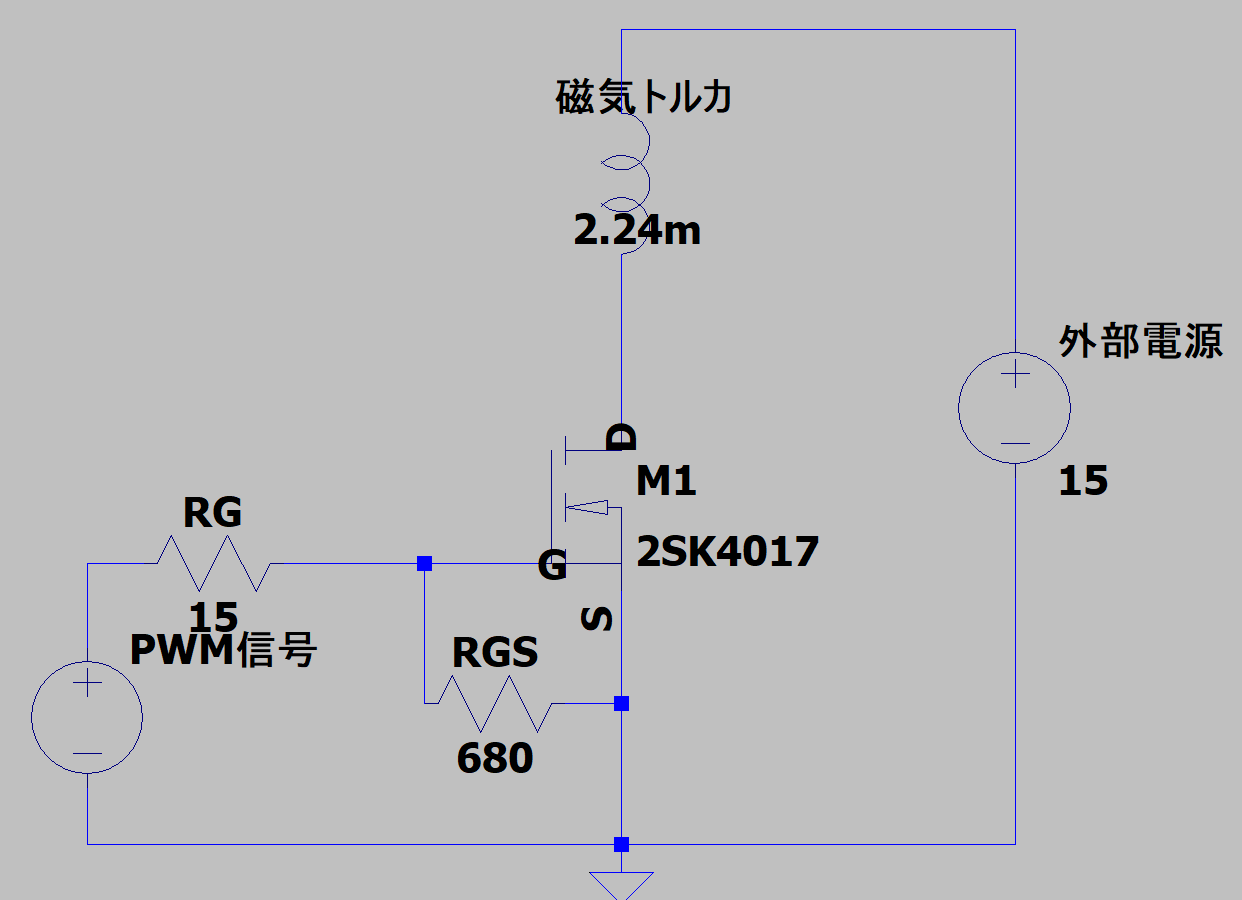
\includegraphics[scale=0.3]{./figure/回路図1.png}
		\caption{初期の磁気トルカの駆動回路}
		\label{fig:cirkit1}
\end{figure}

\begin{figure}[H]
	\centering
		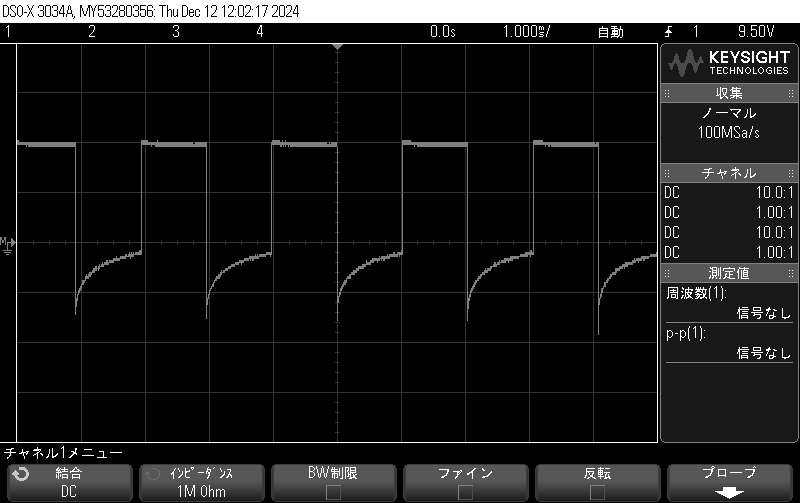
\includegraphics[scale=0.3]{./figure/scope_5.png}
		\caption{初期案}
		\label{fig:osiro1}
\end{figure}


 そこで次に,磁気トルカと並列にダイオードを接続することで逆起電力を防止した.
制作した回路の回路図を図\ref{fig:cirkit}に示す.
具体的には,ON時に磁気トルカに蓄えられたエネルギーを,
ダイオードを通して閉回路となった磁気トルカの抵抗
により消費することにより,逆起電力を防ぐ.

\subsubsection{磁気トルカの電流計算など}

 電流の制御をPWMで行うため,コイルの過渡特性を考慮して電流値の計算を行う必要がある.
一般的にコイルは,インダクタ成分のみでなく抵抗成分も含んでおり,低周波での等価回路は図\ref{fig:touka}のようになる.
よって,LR直列回路の過渡現象を考えればよい.
外部電源の電圧値$E$ [V],抵抗成分$R_L [\Omega]$,インダクタンス$L$ [mH] から求められるFETがONのときの電流の過渡特性は,

\begin{equation}
	i(t) = \frac{E}{R_L}\left(1-e^{-\frac{R_L}{L}t}\right)
\end{equation}

で表される.また,FETがOFFとなったときの時刻を$t_1$ [s] とすると,その後の電流の過渡特性は,

\begin{equation}
	i(t) = \frac{E\left(1-e^{-\frac{R_L}{L}t_1}\right)}{R_L}e^{-\frac{R_L}{L}(t-t_1)}
\end{equation}

となる.さらに$t_2$ [s] 経過し,

\begin{equation}
	i(t) = \frac{E\left(1-e^{-\frac{R_L}{L}t_1}\right)e^{-\frac{R_L}{L}(t_2-t_1)}}{R_L}\left(1-e^{-\frac{R_L}{L}(t-t_1-t_2)}\right)
\end{equation}

というような電流の推移をする.

\begin{table}[H]
	\centering
	\caption{磁気トルカの等価回路}
	\label{table:torquer2}
	\begin{tabular}{|c||c|}
		\hline
		インダクタンス$L$ [mH] & 	82.0 \\ \hline
		抵抗 $R_L$ [$\Omega $] & 18.3 \\ \hline 
	\end{tabular}
\end{table}

\begin{figure}[H]
	\centering
		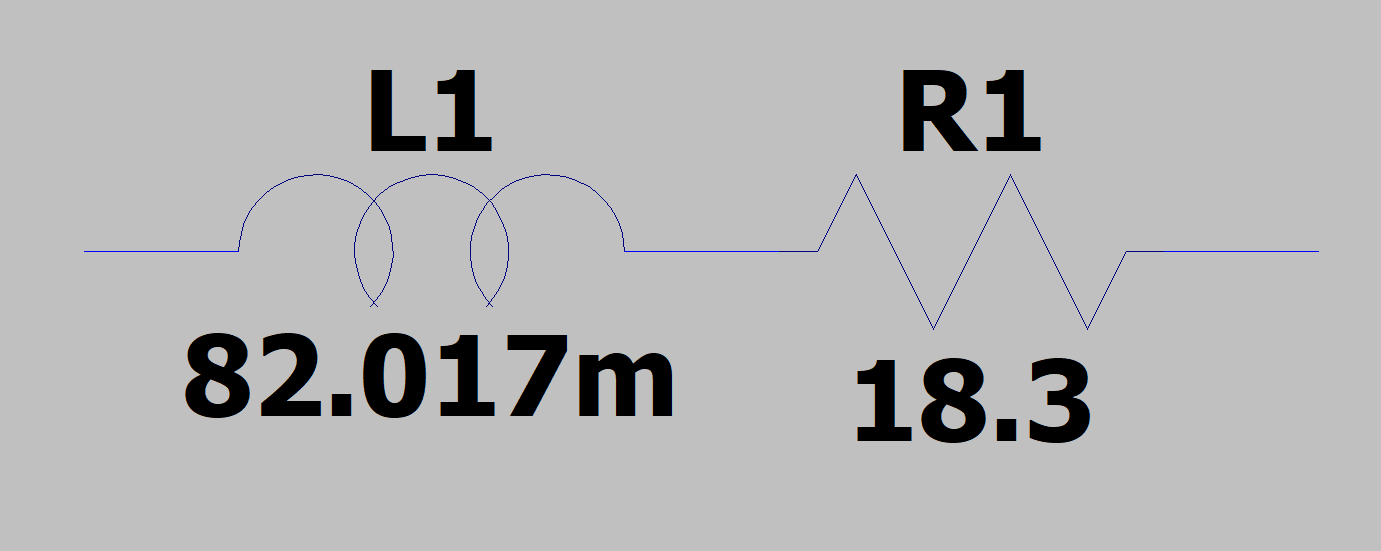
\includegraphics[scale=0.3]{./figure/touka.png}
		\caption{磁気トルカの等価回路}
		\label{fig:touka}
\end{figure}

この電流の推移を,図\ref{fig:cirkit}の回路を用いてduty比50\%でシミュレーションしたグラフを図\ref{fig:current50}に示す.
このように,磁気トルカに電圧E [V] を印加したときの電流を$I_\mathrm{max} [A]$とすると,duty比DのPWM信号で磁気トルカを駆動させたとき,
およその電流を$I(\mathrm{D})=I_\mathrm{max}D [A]$で近似できる. 
そのため電流$I$を流したいときは,$D=\frac{I}{I_\mathrm{max}}$でDuty比を決定する.

\begin{figure}[H]
	\centering
		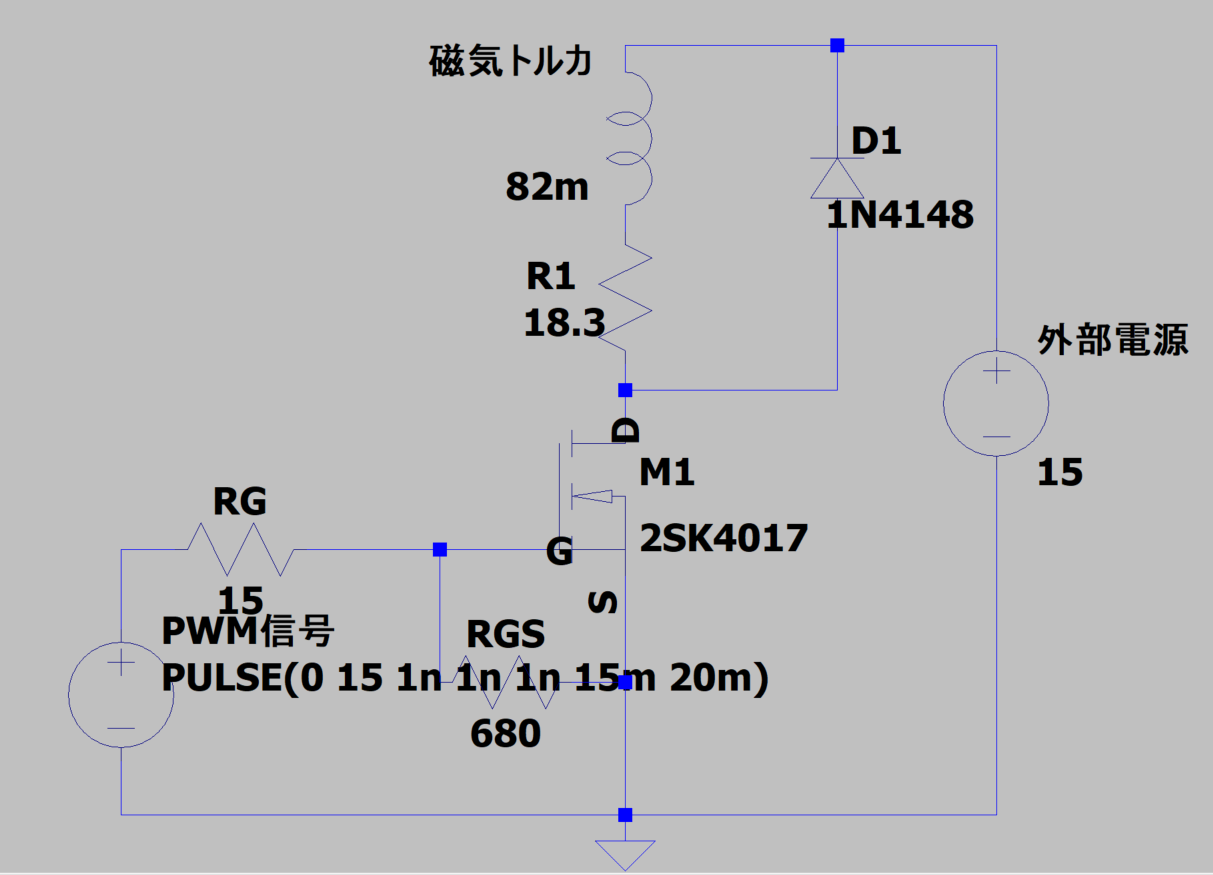
\includegraphics[scale=0.3]{./figure/駆動回路.png}
		\caption{磁気トルカの駆動回路}
		\label{fig:cirkit}
\end{figure}

\begin{figure}[H]
	\centering
		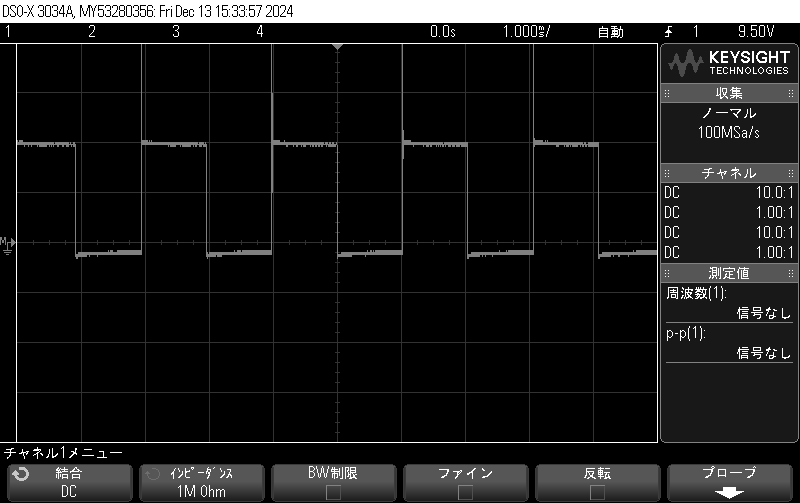
\includegraphics[scale=0.3]{./figure/scope_11.png}
		\caption{磁気トルカに加わる電圧}
		\label{fig:osiro2}
\end{figure}

\begin{figure}[H]
	\centering
		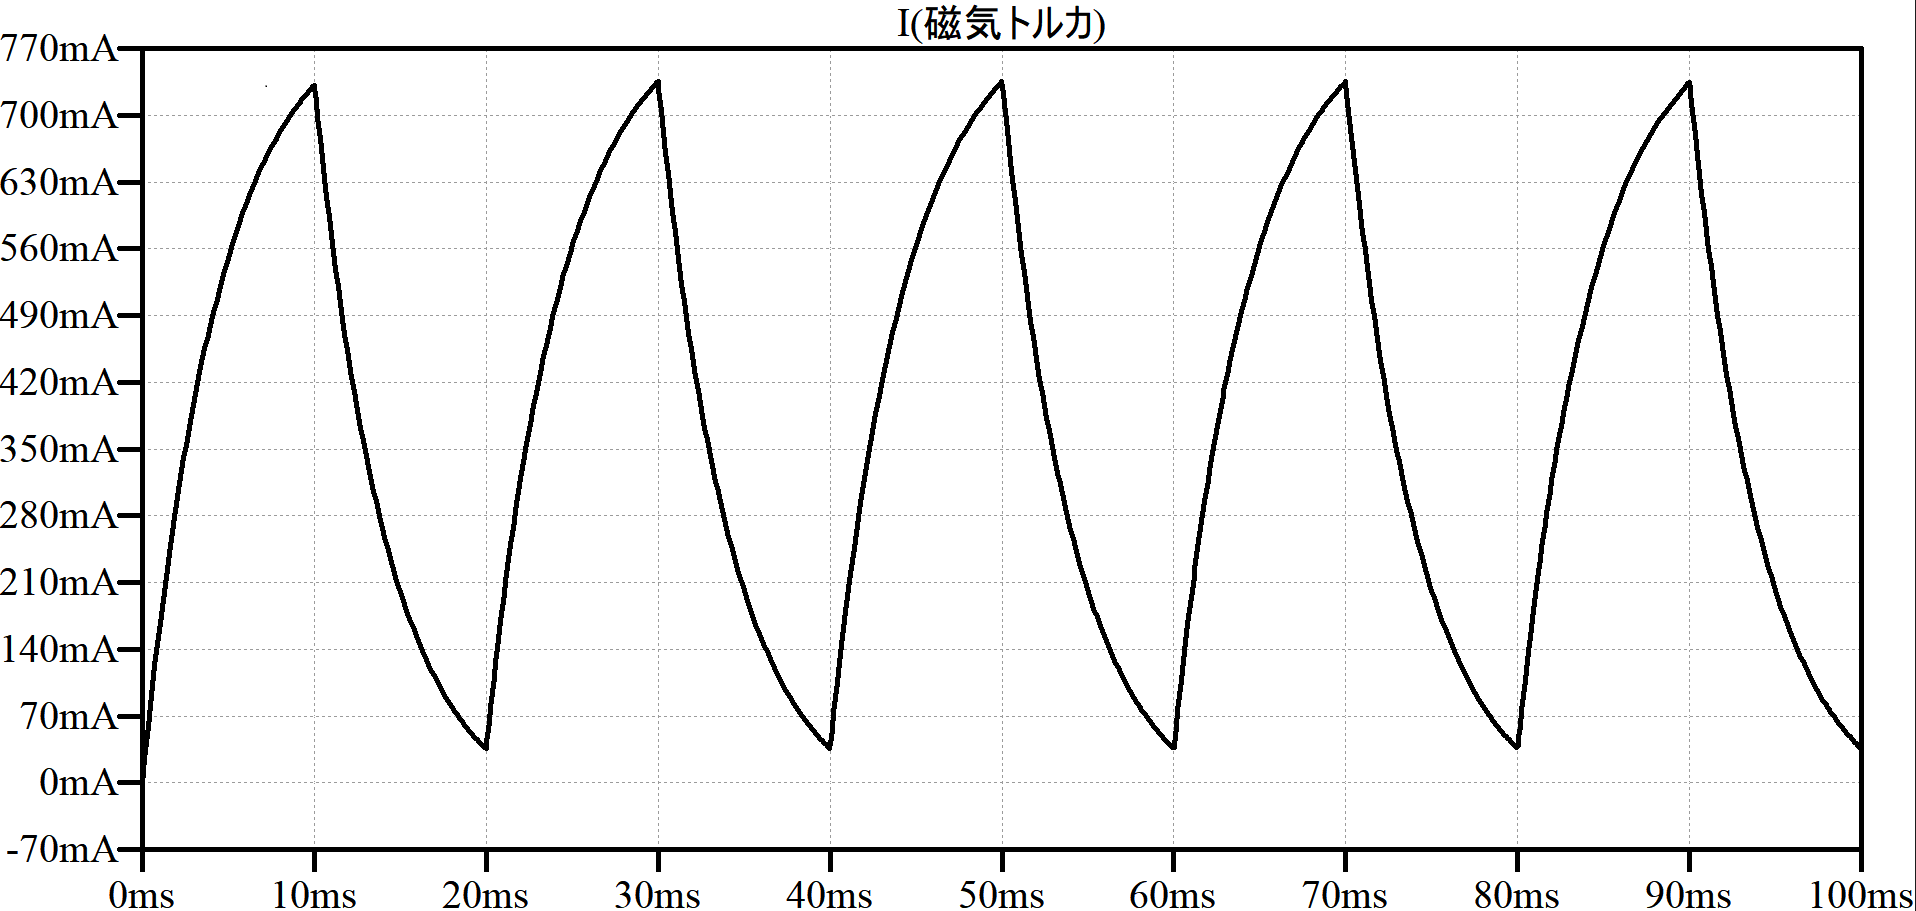
\includegraphics[scale=0.3]{./figure/50current.png}
		\caption{磁気トルカに流れる電流}
		\label{fig:current50}
\end{figure}

 \newpage
% % !TEX root = main.tex
%%%%%%%%%%%%%%%%%%%%%%%%%%%%%%%%%%%%%%%%%%%%%%%%%%%%%%
\section{実験方法および結果}
%%%%%%%%%%%%%%%%%%%%%%%%%%%%%%%%%%%%%%%%%%%%%%%%%%%%%%
 実験装置を図\ref{fig:0deg}の状態から時計回りにに90 [deg] 回転させ,手を離したときの角度推移を観測する.
実験を複数回行い,その平均値の角度推移をグラフにプロットする.また,同時に角速度の推移もプロットし,観測する.
なお,角速度データはノイズが多かったため,csvファイルの角速度データに対して,Pythonの$pykalman$ライブラリを用いてカルマンフィルタを通し,平滑化している.
時刻tにおけるPWM信号のDuty比$D(t)$は,式(3.7)より,
\begin{equation}
	D(t)=\frac{I(t)}{I_{max}}
\end{equation}
とする.

\begin{figure}[h]
	\centering
	\begin{minipage}{0.3\columnwidth}
	  \centering
	  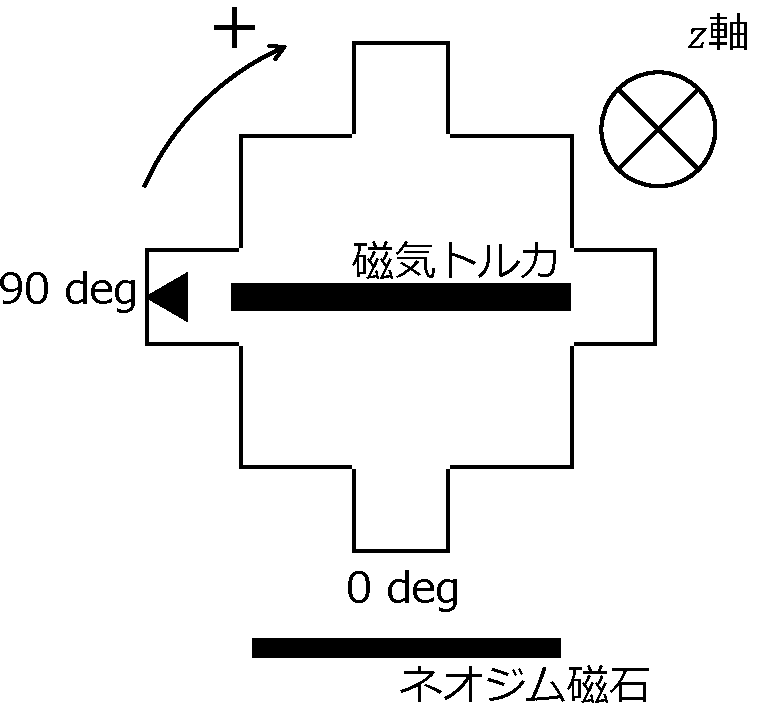
\includegraphics[width=\columnwidth]{./figure/90deg-crop.pdf}
	  \subcaption{角度}
	  \label{fig:90deg}
	\end{minipage}
	\hspace{5mm}
	\begin{minipage}{0.3\columnwidth}
	  \centering
	  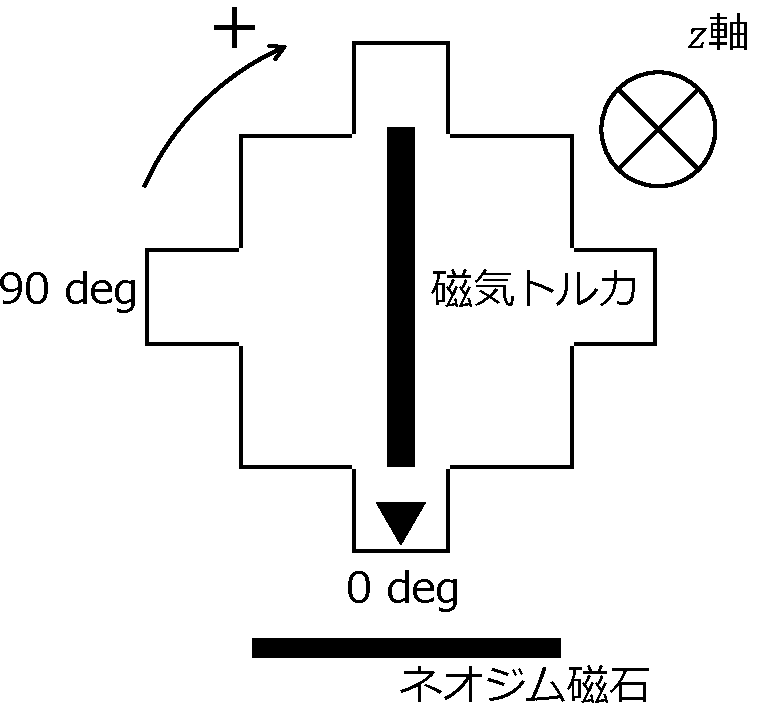
\includegraphics[width=\columnwidth]{./figure/0deg-crop.pdf}
	  \caption{角速度}
	  \label{fig:0deg}
	\end{minipage}
	\caption{Duty比50\%としたとき}
	\label{fig:method}
  \end{figure}

\subsection{Duty比100\%・Duty比50\%による制御}
\subsubsection{実験方法}
 PWM信号のDuty比を,50\%と100\%として実験を行う.


\subsubsection{実験結果}
 Duty比を50\%としたときの結果を図\ref{fig:duty50deg},図\ref{fig:duty50degpers}に,100\%としたときの結果を図\ref{fig:duty100deg},図\ref{fig:duty100degpers}に示す.
図に示すようにオーバーシュートが大きく,振動回数が2回となっている.
また,磁気トルカに触ると明らかに発熱していた.
発熱を抑えようとすれば整定時間が伸びる傾向にあった.

\begin{figure}[h]
	\centering
	\begin{minipage}{0.43\columnwidth}
	  \centering
	  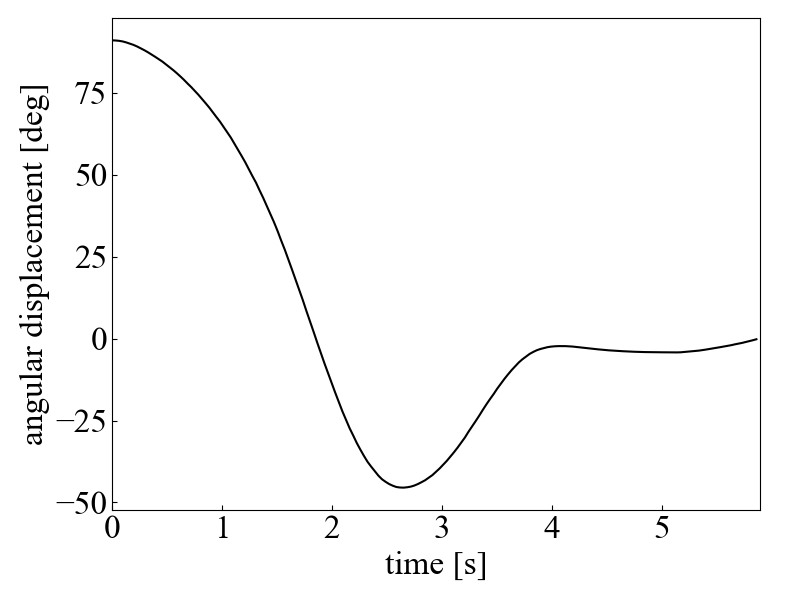
\includegraphics[width=\columnwidth]{./figure/duty50deg.png}
	  \subcaption{角度}
	  \label{fig:duty50deg}
	\end{minipage}
	\hspace{5mm}
	\begin{minipage}{0.43\columnwidth}
	  \centering
	  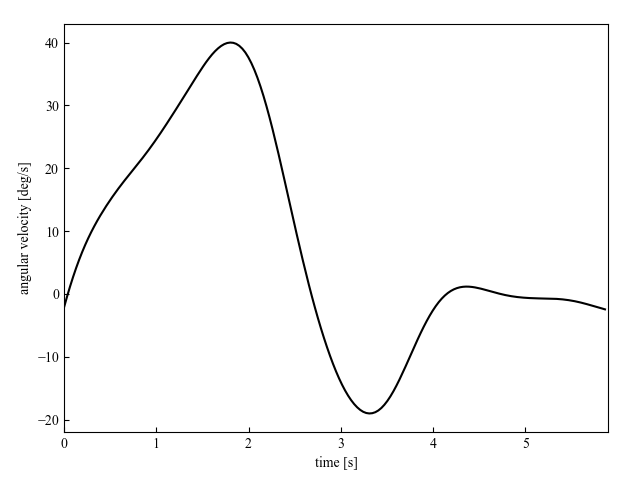
\includegraphics[width=\columnwidth]{./figure/duty50degpers.png}
	  \caption{角速度}
	  \label{fig:duty50degpers}
	\end{minipage}
	\caption{Duty比50\%としたとき}
	\label{fig:Duty50}
  \end{figure}

  \begin{figure}[h]
	\centering
	\begin{minipage}{0.43\columnwidth}
	  \centering
	  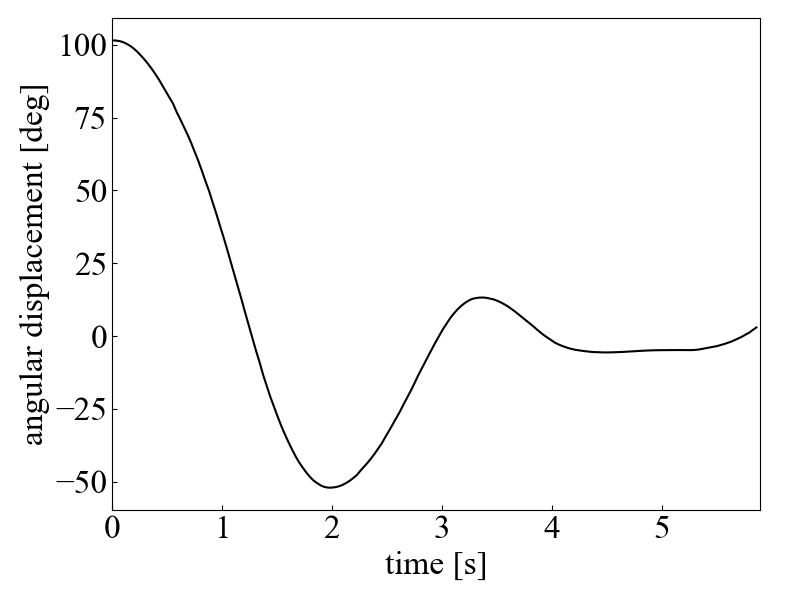
\includegraphics[width=\columnwidth]{./figure/duty100deg.png}
	  \subcaption{角度}
	  \label{fig:duty100deg}
	\end{minipage}
	\hspace{5mm}
	\begin{minipage}{0.43\columnwidth}
	  \centering
	  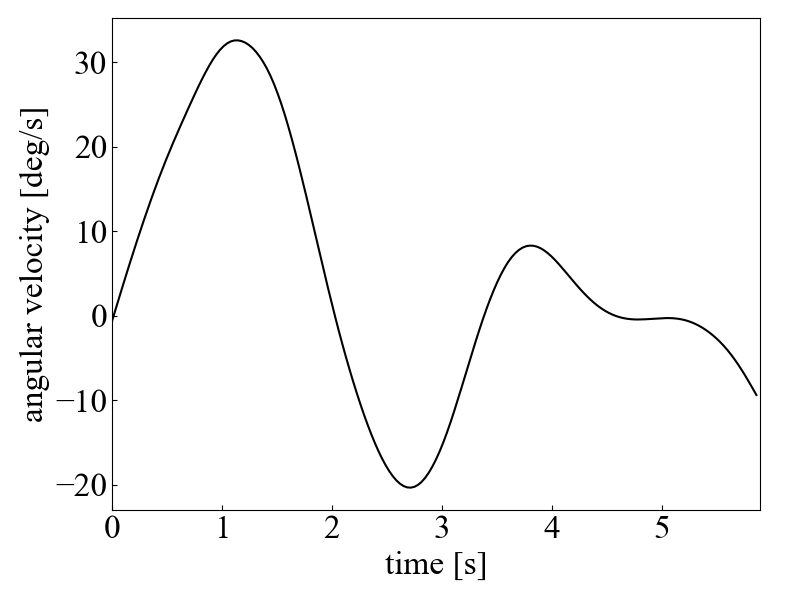
\includegraphics[width=\columnwidth]{./figure/duty100degpers.png}
	  \subcaption{角速度}
	  \label{fig:duty100degpers}
	\end{minipage}
	\caption{Duty比を100\%としたとき}
  \end{figure}

\newpage

\subsection{P制御}
\subsubsection{実験方法}
 Pコントローラを$I(t) = k_P |\theta(t)|$とし,実験を行う.

\subsubsection{実験結果}
 何度か実験を行って$k_P$を調整し,$k_P=0.05$としたときの結果を図\ref{fig:Pdeg},図\ref{fig:Pdegpers}に示す.
整定時間は3.8 s ,定常偏差は2.78 deg であった.

\begin{figure}[h]
	\centering
	\begin{minipage}{0.43\columnwidth}
	  \centering
	  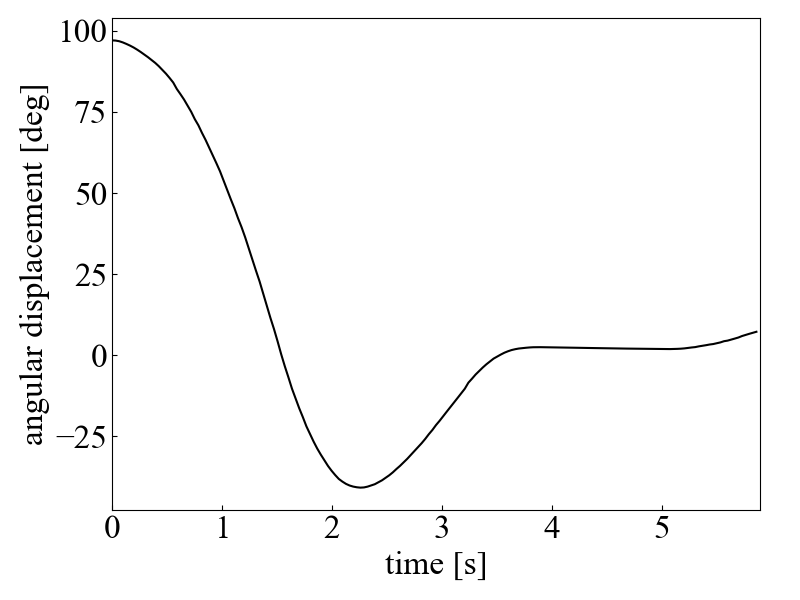
\includegraphics[width=\columnwidth]{./figure/Pdeg.png}
	  \subcaption{角度}
	  \label{fig:Pdeg}
	\end{minipage}
	\hspace{5mm}
	\begin{minipage}{0.43\columnwidth}
	  \centering
	  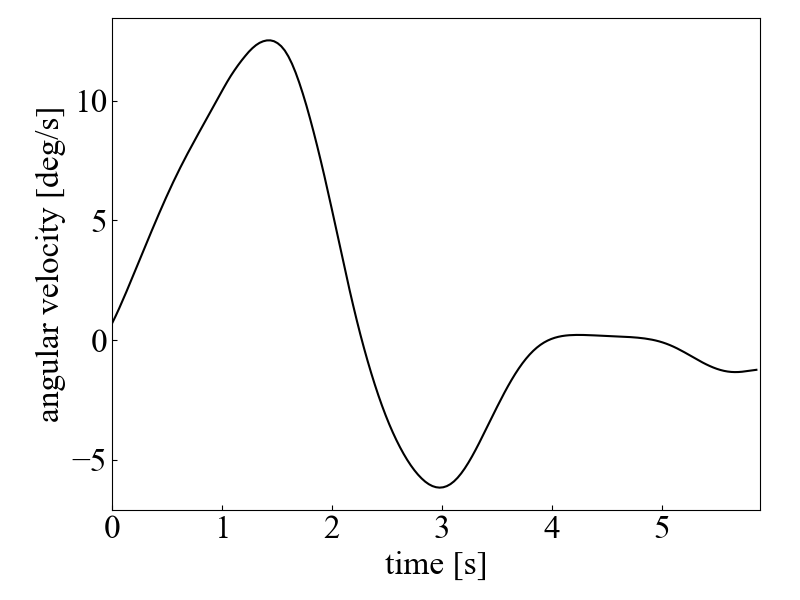
\includegraphics[width=\columnwidth]{./figure/Pdegpers.png}
	  \subcaption{角速度}
	  \label{fig:Pdegpers}
	\end{minipage}
	\caption{P制御}
	\label{fig:P}
  \end{figure}

\newpage

\subsection{PD制御}
\subsubsection{実験方法}
 Pコントローラを$I(t) = k_P |\theta(t)| + k_D|\frac{d\theta(t)}{dt}|$とする.
なお,$\frac{d\theta(t)}{dt}$は,プログラムの1ループ前の角度を$\theta_\mathrm{pre}(t)$とし,$\frac{d\theta(t)}{dt} = \theta(t)-\theta_\mathrm{pre}(t)$で近似する.
\subsubsection{実験結果}
 何度か実験を行ってゲインを調整し,$k_P=0.03$,$k_P=0.05$としたときの結果を図\ref{fig:PDdeg},図\ref{fig:PDdegpers}に示す.
整定時間は4.0 s ,定常偏差は-21.3 deg であった.
\begin{figure}[h]
	\centering
	\begin{minipage}{0.43\columnwidth}
	  \centering
	  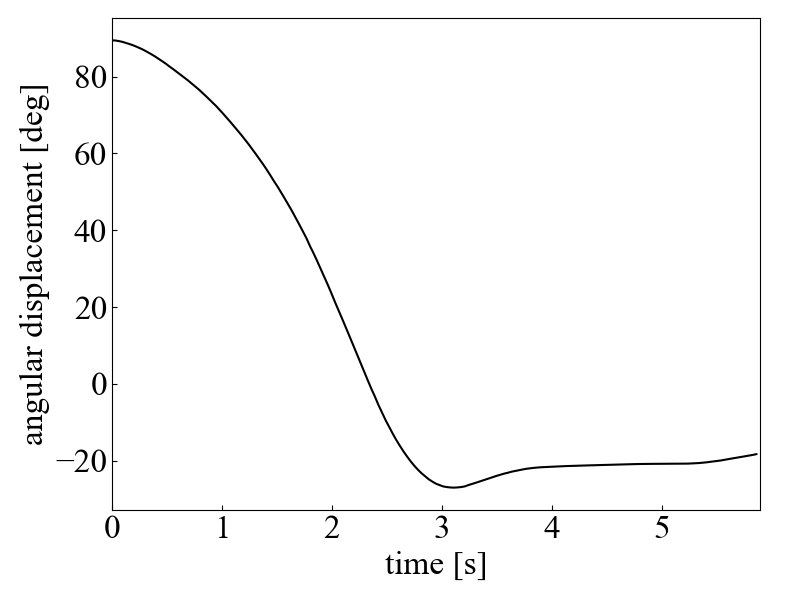
\includegraphics[width=\columnwidth]{./figure/PDdeg.png}
	  \subcaption{角度}
	  \label{fig:PDdeg}
	\end{minipage}
	\hspace{5mm}
	\begin{minipage}{0.43\columnwidth}
	  \centering
	  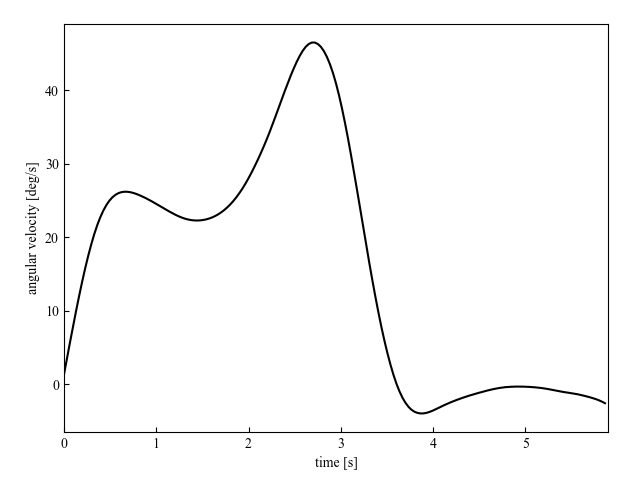
\includegraphics[width=\columnwidth]{./figure/PDdegpers.png}
	  \subcaption{角速度}
	  \label{fig:PDdegpers}
	\end{minipage}
	\caption{PD制御}
	\label{fig:PD}
  \end{figure}

\subsection{B-dot制御則}
\subsubsection{実験方法}
 搭載する磁気トルカが1つであるので,目標磁気モーメントは$M=-k_bB_y\omega_z$である.
$|M|=nIS$より,コントローラを$I=\frac{-k_bB_y\omega_z}{nS}$として実験を行う.

\subsubsection{実験結果}
 $k_b=0.02,k_b=0.05,k_b=0.15$としたときの結果を図\ref{fig:bdotdeg},図\ref{fig:bdotdegpers}に示す.
整定時間は3.0 s ,定常偏差は-13.4 deg であった.

\begin{figure}[h]
	\centering
	\begin{minipage}{0.43\columnwidth}
	  \centering
	  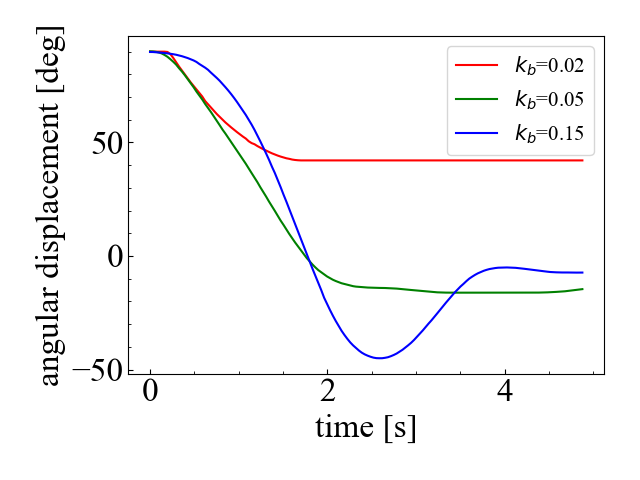
\includegraphics[width=\columnwidth]{./figure/kb5deg.png}
	  \subcaption{角度}
	  \label{fig:bdotdeg}
	\end{minipage}
	\hspace{5mm}
	\begin{minipage}{0.43\columnwidth}
	  \centering
	  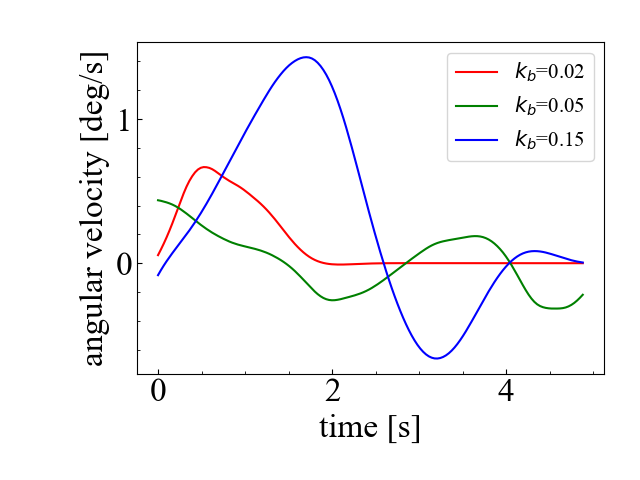
\includegraphics[width=\columnwidth]{./figure/kb5degpers.png}
	  \subcaption{角速度}
	  \label{fig:bdotdegpers}
	\end{minipage}
	\caption{B-dot制御則}
	\label{fig:bdot}
\end{figure}

\newpage

\subsection{クロスプロダクト則}
\subsubsection{実験方法}
 目標磁気モーメントが$M = \frac{K_x c_z + k_x \omega_z}{B_y}$であるので,
コントローラを$I=\frac{K_x c_z + k_x \omega_z}{nSB_y}$として実験を行う.

\subsubsection{実験結果}
 $K_x=0.04$,$k_x=0.03$としたときの結果を図\ref{fig:crossdeg},図\ref{fig:crossdegpers}に示す.
整定時間は3.8 s ,定常偏差は0.1 deg であった.

\begin{figure}[h]
	\centering
	\begin{minipage}{0.43\columnwidth}
	  \centering
	  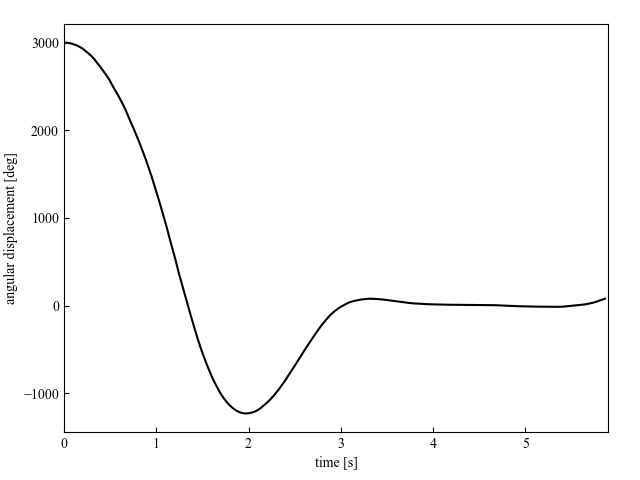
\includegraphics[width=\columnwidth]{./figure/crossdeg.png}
	  \subcaption{角度}
	  \label{fig:crossdeg}
	\end{minipage}
	\hspace{5mm}
	\begin{minipage}{0.43\columnwidth}
	  \centering
	  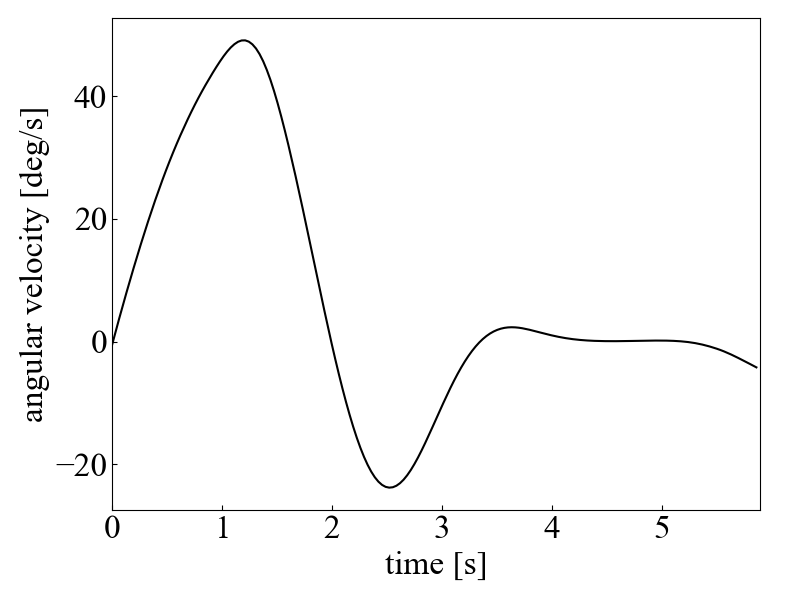
\includegraphics[width=\columnwidth]{./figure/crossdegpers.png}
	  \subcaption{角速度}
	  \label{fig:crossdegpers}
	\end{minipage}
	\caption{クロスプロダクト則}
	\label{fig:cross}
\end{figure}


\subsection{考察}
 各結果の整定時間,定常偏差を表\ref{table:result}に示す.
この表から,整定時間に基づいて評価すればB-dot制御則が最適であり,
定常偏差に基づいて評価すればクロスプロダクト則が最も優れた制御則となる結果を得た.
P,PD,クロスプロダクト則は,制御量が角度であるのに対して積分要素を含まないため,ゲインの組み合わせによっては定常偏差が残る.
B-dot制御則は制御量が角速度であるため,定常偏差が残っている.

\begin{table}[H]
	\centering
	\caption{実験結果}
	\label{table:result}
	\begin{tabular}{|c||c|c|c|c|c|c|}
		\hline
		 & 50\% & 100\% & P制御 & PD制御 & B-dot制御則 & クロスプロダクト制御則 \\ \hline
		整定時間T [s] & 4.1 & 4.3 & 3.8 & 4.0 & 3.0 & 3.8 \\ \hline
		定常偏差$\theta$ [deg] & 0 & 0 & 2.78 & -21.3 & -13.4 & 0.1 \\ \hline
	\end{tabular}
\end{table}


\newpage
\section{結論}
\subsection{本研究のまとめ}
 本研究では,人工衛星の模型や実験システムを新規に作製して,磁気トルカによる姿勢制御を検証した.

B-dot制御則については,制御理論の特徴が現れる結果となった.
しかし,PD制御・クロスプロダクト則についてはゲイン設定の余地があり,

本研究で作製した実験装置は,転がり軸受の摩擦や外部電源との接続といった部分で宇宙空間の環境とは程遠く,


先行研究では,想定される人工衛星の大きさの違いや,磁気トルカでの検証を行われていなかったため,超小型人工衛星の,特に磁気トルカに注目して実験装置を作製し,検証を行った.定常偏差を無視すればB-dot制御則が,定常偏差を考慮すればクロスプロダクト則が最も性能の良い制御理論となる結果を得た.
\subsection{今後の展望}

 摩擦の影響がない宇宙空間を想定すると,積分要素が含まれていなくても定常偏差は残らない.転がり軸受の工夫等により摩擦をさらに軽減できれば,PD制御・クロスプロダクト則は定常偏差が残らず,B-dot制御則との役割の違いが現れ,評価が変わる可能性がある. 

 今回は磁気トルカを1本のみ用いて検証を行った.しかし実際の人工衛星の姿勢制御では,1軸に対して磁気トルカを2本用いて姿勢制御を行っていることも多いため,磁気トルカをもう1本増やした検証も必要であると考える.

また,作製した模型の質量,大きさなどから宇宙空間での挙動のシミュレーションを行い,その結果との類似点・相違点を比較して改良点を考える. \newpage

%%%%%%%%%%%%%%%%%%%%%%%%%%%%%%%%%%%%%%%%%%%%%%%%%%%%%%%%%%%%%%%%%%%%%%%%%%%%%
%%%%%% 参考文献 %%%%%%%%%%%%%%%%%%%%%%%%%%%%%%%%%%%%%%%%%%%%%%%%%%%%%%%%%%%
%%%%%%%%%%%%%%%%%%%%%%%%%%%%%%%%%%%%%%%%%%%%%%%%%%%%%%%%%%%%%%%%%%%%%%%%%%%%%
% !TEX root = main.tex
%%%%%%%%%%%%%%%%%%%%%%%%%%%%%%%%%%%%%%%%%%%%%%%%%%%%%%%%%%%%%%%%%%%%%%%%
\begin{center}
\section*{\kintou{5zw}{参考文献}}                      %% ここに番号をつけない
\vspace*{-2zh}
\end{center}
\addcontentsline{toc}{section}{参考文献} %% 目次に番号をつけない
%%%%%%%%%%%%%%%%%%%%%%%%%%%%%%%%%%%%%%%%%%%%%%%%%%%%%%%%%%%%%%%%%%%%%%%%

\begin{thebibliography}{99}
\bibitem{bdot}
	Goddard Space Flight Center:
	Flight Mechanics Symposium 1997: Proceedings of a Conference Sponsored by NASA Goddard
	 Space Flight Center at Goddard Space Flight Center, Greenbelt, Maryland, May 19-21, 1997,
	 IICA Biblioteca Venezuela (1997)

\bibitem{bdot}
	Kikuko Miyata and Jozef C. van der Ha:
	AT TI TUDE CON TROL BY MAG NETIC TORQUER,
	Advances in the Astronautical Sciences (2009)

\bibitem{Sato1}
	佐藤太郎:
	高等専門学校における一般科目と専門科目,
	京都出版 (2018)
	\textcolor{red}{\quad\cdotfill\ 本の場合}
	
\bibitem{Suzuki1}
	鈴木次郎,高橋三郎:
	高等専門学校と大学の違い,
	電子制御学会論文誌,
	Vol.~25, No.~13, 123/130 (2017)
	\textcolor{red}{\quad\cdotfill\ 学会誌論文の場合}
	
\bibitem{Tanaka1}
	田中史朗,伊藤五郎,渡辺花子:
	高専における就職活動,
	電気電子工学講演会資料,
	543/546 (2016)
	\textcolor{red}{\quad\cdotfill\ 講演会等資料(ページが記載されているもの)の場合}
	
\bibitem{Yamamoto1}
	山本一二三,中村五十六:
	高専における就職活動,
	メカトロニクス講演会資料,
	全 4 頁 (2016)
	\textcolor{red}{\quad\cdotfill\ 講演会等資料(ページが記載されていないもの)の場合}
	
\bibitem{Nakamura1}
	中村十三子:
	機械加工と実習工場,
	平成 29 年度舞鶴工業高等専門学校機械工学科卒業論文 (2018)
	\textcolor{red}{\quad\cdotfill\ 卒業論文の場合}
	
\bibitem{Sato2}
	T.~Sato: 
	General Subjects and Special subjects at National Institute of Technology, 
	Kyoto Publishing (2018)
	
\bibitem{Suzuki2}
	J.~Suzuki and S.~Takahashi: 
	Difference between National Institute of Technology and Universities, 
	Journal of the Electronic Control Society, 
	Vol.~25, No.~13, 123/130 (2017)
	
\bibitem{Tanaka2}
	S.~Tanaka, G.~Ito and H.~Watanabe: 
	Job Hunting in NIT, 
	Proceedings of Conference on Electrical and Electronics Engineering, 
	543/546 (2016)
	
\bibitem{Yamamoto2}
	H.~Yamamoto and I.~Nakamura: 
	Job Hunting in NIT, 
	Proceedings of Mechatoronics Conference, 
	4 pages (2016)
	
\bibitem{NIT1}
	舞鶴高専ホームページ:
	\url{http://www.maizuru-ct.ac.jp}
\end{thebibliography}
% ******************************************* \newpage

%%%%%%%%%%%%%%%%%%%%%%%%%%%%%%%%%%%%%%%%%%%%%%%%%%%%%%%%%%%%%%%%%%%%%%%%%%%%%
%%%%%% 謝辞 %%%%%%%%%%%%%%%%%%%%%%%%%%%%%%%%%%%%%%%%%%%%%%%%%%%%%%%%%%%%%%%
%%%%%%%%%%%%%%%%%%%%%%%%%%%%%%%%%%%%%%%%%%%%%%%%%%%%%%%%%%%%%%%%%%%%%%%%%%%%%
% !TEX root = main.tex
%%%%%%%%%%%%%%%%%%%%%%%%%%%%%%%%%%%%%%%%%%%%%%%%%%%%%%%%%%%%%%%%%%%%%%%%
\begin{center}
\section*{\kintou{2.5zw}{謝辞}}                      %% ここに番号をつけない
\vspace*{-2zh}
\end{center}
\addcontentsline{toc}{section}{謝辞} %% 目次に番号をつけない
%%%%%%%%%%%%%%%%%%%%%%%%%%%%%%%%%%%%%%%%%%%%%%%%%%%%%%%%%%%%%%%%%%%%%%%%

 本研究を進めるにあたり,多くの方々にご指導ご鞭撻を賜りました.
指導教員の西佑介教授からは多大なご指導を賜り,数々の助言を頂きました.
また,編入学試験に際して,面接練習や受験勉強の場を提供して頂きました.心より感謝いたします.\\
 電子制御工学科教員の仲川力教授には,ガウスメータを貸与していただき,
考察を深めることができました.心より感謝いたします.\\
 本科5年の野口史遠氏には,Arduinoや回路制作で行き詰まった際に
多くの助言を頂きました.心より感謝いたします.\\
 専攻科1年の三宅航希氏と,本科5年の正木律氏には,特に電子回路について助言をいただき,
回路の改良にご助力頂きました.心より感謝いたします.\\
 本科5年の神田大訓氏には,研究内容は異なるものの,実験に対するひたむきな姿勢に感化されることもありました.
心より感謝いたします.\\
 本科5年の澤田一理氏には,卒研発表のスライドにおいて自分の視点にはない鋭い指摘を頂き,
よりよい発表スライドを作成できました.心より感謝いたします.\\
 本科5年の櫻井蒼真氏には,卒業研究の中間発表の練習に際して,発表に関する改善点を指摘いただき,
満足のいく発表ができました.心より感謝いたします.\\
 本科5年の林巧巳氏には,編入学試験の勉強について,度々議論を交わしていただき,互いに高めあうことができました.
心より感謝いたします.\\
 最後に,研究や日頃の生活において,有形無形の援助をしていただいた舞鶴高専電子制御工学科教員
の皆様,および生活を支えてくださった家族と友人に心より感謝いたします.\\ \newpage

%%%%%%%%%%%%%%%%%%%%%%%%%%%%%%%%%%%%%%%%%%%%%%%%%%%%%%%%%%%%%%%%%%%%%%%%%%%%%
%%%%%% 付録 %%%%%%%%%%%%%%%%%%%%%%%%%%%%%%%%%%%%%%%%%%%%%%%%%%%%%%%%%%%%%%%
%%%%%%%%%%%%%%%%%%%%%%%%%%%%%%%%%%%%%%%%%%%%%%%%%%%%%%%%%%%%%%%%%%%%%%%%%%%%%
% !TEX root = main.tex
%////////////////////////////////////////////////////////
\begin{center}
\section*{\kintou{2.5zw}{付録}}                      %% ここに番号をつけない
\vspace*{-2zh}
\end{center}
\addcontentsline{toc}{section}{付録} %% 目次に番号をつけない
\appendix

\setcounter{equation}{0}
\setcounter{figure}{0}
\setcounter{table}{0}

\makeatletter
     \renewcommand{\theequation}{%
          A.\arabic{equation}}
     \@addtoreset{equation}{section}
\makeatother

\makeatletter
     \renewcommand{\thetable}{%
          A.\arabic{table}}
     \@addtoreset{table}{section}
\makeatother

\makeatletter
     \renewcommand{\thefigure}{%
          A.\arabic{figure}}
     \@addtoreset{figure}{section}
\makeatother

% ================================================
\makeatletter
     \renewcommand{\thesubsection}{%
          A.\arabic{subsection}}
     \@addtoreset{subsection}{section}
\makeatother

\makeatletter
     \renewcommand{\thesubsubsection}{%
          A.\arabic{subsection}.\arabic{subsubsection}}
     \@addtoreset{subsubsection}{section}
\makeatother

% ================================================
\makeatletter
     \renewcommand{\thetheorem}{%
          A.\arabic{theorem}}
     \@addtoreset{theorem}{section}
\makeatother

\makeatletter
     \renewcommand{\thedefinition}{%
          A.\arabic{definition}}
     \@addtoreset{definition}{section}
\makeatother

\makeatletter
     \renewcommand{\thelemma}{%
          A.\arabic{lemma}}
     \@addtoreset{lemma}{section}
\makeatother

\makeatletter
     \renewcommand{\thelstlisting}{%
          {\bf{A.\arabic{lstlisting}}}}
     \@addtoreset{lstlisting}{section}
\makeatother






%////////////////////////////////////////////////////////

%%%%%%%%%%%%%%%%%%%%%%%%%%%%%%%%%%%%%%%%%%%%%%%%%%%%%%
\subsection{ちちち}
%%%%%%%%%%%%%%%%%%%%%%%%%%%%%%%%%%%%%%%%%%%%%%%%%%%%%%
 以下に,本研究で使用したArduino用のC++プログラムを示す.
\begin{lstlisting}
    #include <Wire.h>
#include <SD.h>
#include <Adafruit_Sensor.h>
#include <Adafruit_BNO055.h>
#include <utility/imumaths.h>
#define PWM 9
#define VMAX 15.0f
#define RESISTER 18.37

double T=0.0327438; //実行時間
double e_pre = 0.0; // 微分の近似計算のための初期値
double de = 0.0; 
double ie = 0.0;    // 積分の近似計算のための初期値
const int analogWriteStep = 255;
int dutyRatio = 80; //duty比[%]
double angle[3]={-1000,-1000,-1000};
double magne[3]={-1000,-1000,-1000};
double gyro[3]={-1000,-1000,-1000};
double bdot[3]={0,0,0};
unsigned long int time;
const int chipSelect = 10;
double kb = 0.00005;
double kp = 0.007;
double kd = 0.004;
double ki = 0.001;
double current = 0;
double voltage = 0;
//string型宣言
String datastr = "";
// Check I2C device address and correct line below (by default address is 0x29 or 0x28)
//                                   id, address
Adafruit_BNO055 bno = Adafruit_BNO055(55, 0x28, &Wire);

void setup(void)
{
  pinMode(10, OUTPUT);
  pinMode(9,OUTPUT);
  Serial.begin(115200);
  Serial.println("Orientation Sensor Test"); Serial.println("");
  //センサの初期化
  if (!bno.begin())
  {
    /* There was a problem detecting the BNO055 ... check your connections */
    Serial.print("Ooops, no BNO055 detected ... Check your wiring or I2C ADDR!");
    while (1);
  }
  //SDカードの初期化
  if (!SD.begin(chipSelect)) {
    Serial.println("SD card initialization failed!");
    while (1); // 初期化に失敗したら停止
  }
  Serial.println("initialization done.");
}

void loop(void){
  //could add VECTOR_ACCELEROMETER, VECTOR_MAGNETOMETER,VECTOR_GRAVITY...
  sensors_event_t orientationData , angVelocityData , linearAccelData, magnetometerData, accelerometerData, gravityData;
  bno.getEvent(&orientationData, Adafruit_BNO055::VECTOR_EULER);
  bno.getEvent(&angVelocityData, Adafruit_BNO055::VECTOR_GYROSCOPE);
  bno.getEvent(&linearAccelData, Adafruit_BNO055::VECTOR_LINEARACCEL);
  bno.getEvent(&magnetometerData, Adafruit_BNO055::VECTOR_MAGNETOMETER);
  bno.getEvent(&accelerometerData, Adafruit_BNO055::VECTOR_ACCELEROMETER);
  bno.getEvent(&gravityData, Adafruit_BNO055::VECTOR_GRAVITY);

  //センサの値を取得
  returnEvent(&orientationData,angle);
  returnEvent(&magnetometerData,magne);
  returnEvent(&angVelocityData,gyro);

  //Bdot制御則の計算
  bdot[0]=magne[1]*gyro[2]-magne[2]*gyro[1];
  bdot[1]=magne[0]*gyro[2]-magne[2]*gyro[0];
  bdot[2]=magne[0]*gyro[1]-magne[1]*gyro[0];

  //目標角度を0[deg]とする
  double e = angle[0];
  if(e > 270){
    e = abs(e - 360);
  }
  de = (e - e_pre)/T;  
  ie = ie + (e + e_pre)*T/2;

  //B-dotならコメントアウト
  current = kp*e + ki*ie + kd*de;
  //PIDならコメントアウト
  // current = kb*bdot[0]/0.04935;

  //算出した電流値を電圧値に変換
  voltage = current * RESISTER;
  if(abs(voltage) > VMAX) {
    voltage = VMAX;
  }
  //電圧値をduty比に変換
  int duty = int(abs((voltage / 15.0) * 100.0));
  Serial.print(duty);

  int ledBrightness = analogWriteStep * duty / 100.0f;
  analogWrite( 9, ledBrightness );

  //値をstring型に
  datastr = String(angle[0]);
  for (int i = 0; i < 3; i++){
    datastr += ","+String(magne[i]);
  }
  datastr += ","+String(gyro[2]);
  //csvファイルのopen
  File angFile = SD.open("LOG.CSV", FILE_WRITE);
  //書き込み
  if (angFile) {
    angFile.println(datastr);
    angFile.close(); // ファイルを閉じる
    Serial.println("Write successful.");
  } else {
    Serial.println("Error opening test.txt for writing.");
  }
  e_pre = e;
}

//センサの値を返す
void returnEvent(sensors_event_t* event,double tmp[3]) {
  double x = -1000000, y = -1000000 , z = -1000000; //dumb values, easy to spot problem
  if (event->type == SENSOR_TYPE_ACCELEROMETER) {
    Serial.print("Accl:");
    x = event->acceleration.x;
    y = event->acceleration.y;
    z = event->acceleration.z;
  }
  else if (event->type == SENSOR_TYPE_ORIENTATION) {
    // Serial.print("orient:");
    x = event->orientation.x;
    y = event->orientation.y;
    z = event->orientation.z;
  }
  else if (event->type == SENSOR_TYPE_MAGNETIC_FIELD) {
    // Serial.print("Mag:");
    x = event->magnetic.x;
    y = event->magnetic.y;
    z = event->magnetic.z;
  }
  else if (event->type == SENSOR_TYPE_GYROSCOPE) {
    // Serial.print("Gyro:");
    x = event->gyro.x;
    y = event->gyro.y;
    z = event->gyro.z;
  }
  else if (event->type == SENSOR_TYPE_ROTATION_VECTOR) {
    Serial.print("Rot:");
    x = event->gyro.x;
    y = event->gyro.y;
    z = event->gyro.z;
  }
  else if (event->type == SENSOR_TYPE_LINEAR_ACCELERATION) {
    Serial.print("Linear:");
    x = event->acceleration.x;
    y = event->acceleration.y;
    z = event->acceleration.z;
  }
  else if (event->type == SENSOR_TYPE_GRAVITY) {
    Serial.print("Gravity:");
    x = event->acceleration.x;
    y = event->acceleration.y;
    z = event->acceleration.z;
  }
  else {
    Serial.print("Unk:");
  }

  tmp[0]=x;
  tmp[1]=y;
  tmp[2]=z;
}


\end{lstlisting}


\end{document}